
%(BEGIN_QUESTION)
% Copyright 2010, Tony R. Kuphaldt, released under the Creative Commons Attribution License (v 1.0)
% This means you may do almost anything with this work of mine, so long as you give me proper credit

The {\it load cell} assembly for one leg of a weight-based level measurement system uses two strain gauges connected to a Wheatstone bridge circuit.  One strain gauge senses the applied force, while the other merely compensates for temperature changes:

$$\includegraphics[width=15.5cm]{i03678x01.eps}$$

Calculate the magnitude and polarity of the voltage output (between points A and B) of this bridge circuit when the strain gauge's resistance is 6.3 k$\Omega$ and the ``dummy'' gauge's resistance is 5.9 k$\Omega$:

\vskip 10pt

$V_{out}$ = \underbar{\hskip 50pt} millivolts

\underbar{file i03678}
%(END_QUESTION)





%(BEGIN_ANSWER)

$V_{out}$ = \underbar{\bf 1.638} millivolts, point A being more positive than point B.

\vskip 10pt

5 points for correct magnitude, 5 points for correct polarity.

%(END_ANSWER)





%(BEGIN_NOTES)

{\bf This question is intended for exams only and not worksheets!}.

%(END_NOTES)

